\section{Introduction}
Some text followed by bullets.
\begin{itemize}
\item This is an item
\item And another
\end{itemize}
Now we will use numbers.
\begin{enumerate}
\item There should be a number
\item And another
\end{enumerate}
\subsection{Subsection}
Let's have a subsection
\subsubsection{Subsubsection}
And a subsubsection with figures
\begin{figure}[H]
  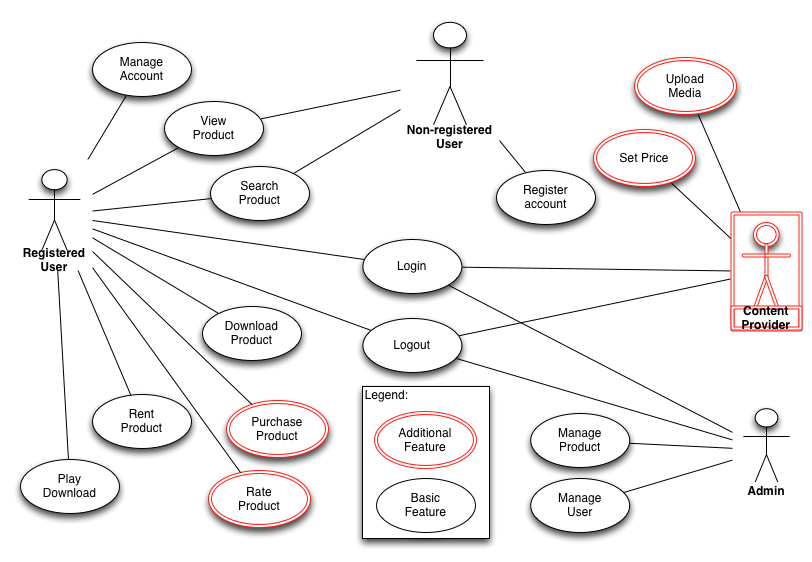
\includegraphics[width=\textwidth]{illustrations/UseCase_ver1.png}
  \caption{Usecase version 1.1}
  \label{dailyscrum}
\end{figure}
\begin{figure}[H]
  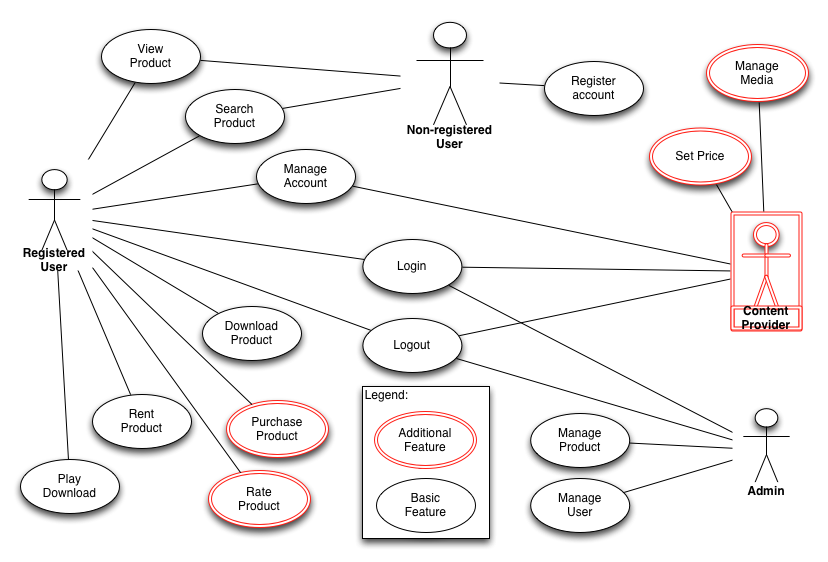
\includegraphics[width=\textwidth]{illustrations/UseCase_ver2.png}
  \caption{Usecase version 2.0}
  \label{burndown}
\end{figure}
\subsubsection{Subsubsection 2}
\textbf{caption} is used as picture description text\\
\textbf{label} is used if one wish to refer to the item at some point\\
\textbf{figure parameter} is used for positioning. It will ignore you, if your wish does not fit well with the text.\\
\begin{table*}[h!]\centering
  \ra{1.3}
  \begin{tabularx}{\textwidth}{@{}rXXl@{}}\toprule
    \textbf{Parameter} & \textbf{Effect}\\
    h & Place the float here, i.e., approximately at the same point it occurs in the source text (however, not exactly at the spot)\\
    t & Position at the top of the page.\\
    b & Position at the bottom of the page.\\
    p & Put on a special page for floats only.\\
    ! & Override internal parameters LaTeX uses for determining "good" float positions.\\
    H & Places the float at precisely the location in the LaTeX code. Requires the float package. This is somewhat equivalent to h!.\\
	\bottomrule
  \end{tabularx}
\end{table*}
\newpage